% Options for packages loaded elsewhere
\PassOptionsToPackage{unicode}{hyperref}
\PassOptionsToPackage{hyphens}{url}
\PassOptionsToPackage{dvipsnames,svgnames,x11names}{xcolor}
%
\documentclass[
  9pt,
]{article}

\usepackage{amsmath,amssymb}
\usepackage{iftex}
\ifPDFTeX
  \usepackage[T1]{fontenc}
  \usepackage[utf8]{inputenc}
  \usepackage{textcomp} % provide euro and other symbols
\else % if luatex or xetex
  \usepackage{unicode-math}
  \defaultfontfeatures{Scale=MatchLowercase}
  \defaultfontfeatures[\rmfamily]{Ligatures=TeX,Scale=1}
\fi
\usepackage{lmodern}
\ifPDFTeX\else  
    % xetex/luatex font selection
  \setmainfont[]{EB Garamond}
  \setsansfont[]{Montserrat}
\fi
% Use upquote if available, for straight quotes in verbatim environments
\IfFileExists{upquote.sty}{\usepackage{upquote}}{}
\IfFileExists{microtype.sty}{% use microtype if available
  \usepackage[]{microtype}
  \UseMicrotypeSet[protrusion]{basicmath} % disable protrusion for tt fonts
}{}
\makeatletter
\@ifundefined{KOMAClassName}{% if non-KOMA class
  \IfFileExists{parskip.sty}{%
    \usepackage{parskip}
  }{% else
    \setlength{\parindent}{0pt}
    \setlength{\parskip}{6pt plus 2pt minus 1pt}}
}{% if KOMA class
  \KOMAoptions{parskip=half}}
\makeatother
\usepackage{xcolor}
\usepackage[margin=20mm,paperwidth=17cm,paperheight=24cm]{geometry}
\setlength{\emergencystretch}{3em} % prevent overfull lines
\setcounter{secnumdepth}{-\maxdimen} % remove section numbering
% Make \paragraph and \subparagraph free-standing
\ifx\paragraph\undefined\else
  \let\oldparagraph\paragraph
  \renewcommand{\paragraph}[1]{\oldparagraph{#1}\mbox{}}
\fi
\ifx\subparagraph\undefined\else
  \let\oldsubparagraph\subparagraph
  \renewcommand{\subparagraph}[1]{\oldsubparagraph{#1}\mbox{}}
\fi


\providecommand{\tightlist}{%
  \setlength{\itemsep}{0pt}\setlength{\parskip}{0pt}}\usepackage{longtable,booktabs,array}
\usepackage{calc} % for calculating minipage widths
% Correct order of tables after \paragraph or \subparagraph
\usepackage{etoolbox}
\makeatletter
\patchcmd\longtable{\par}{\if@noskipsec\mbox{}\fi\par}{}{}
\makeatother
% Allow footnotes in longtable head/foot
\IfFileExists{footnotehyper.sty}{\usepackage{footnotehyper}}{\usepackage{footnote}}
\makesavenoteenv{longtable}
\usepackage{graphicx}
\makeatletter
\def\maxwidth{\ifdim\Gin@nat@width>\linewidth\linewidth\else\Gin@nat@width\fi}
\def\maxheight{\ifdim\Gin@nat@height>\textheight\textheight\else\Gin@nat@height\fi}
\makeatother
% Scale images if necessary, so that they will not overflow the page
% margins by default, and it is still possible to overwrite the defaults
% using explicit options in \includegraphics[width, height, ...]{}
\setkeys{Gin}{width=\maxwidth,height=\maxheight,keepaspectratio}
% Set default figure placement to htbp
\makeatletter
\def\fps@figure{htbp}
\makeatother
\newlength{\cslhangindent}
\setlength{\cslhangindent}{1.5em}
\newlength{\csllabelwidth}
\setlength{\csllabelwidth}{3em}
\newlength{\cslentryspacingunit} % times entry-spacing
\setlength{\cslentryspacingunit}{\parskip}
\newenvironment{CSLReferences}[2] % #1 hanging-ident, #2 entry spacing
 {% don't indent paragraphs
  \setlength{\parindent}{0pt}
  % turn on hanging indent if param 1 is 1
  \ifodd #1
  \let\oldpar\par
  \def\par{\hangindent=\cslhangindent\oldpar}
  \fi
  % set entry spacing
  \setlength{\parskip}{#2\cslentryspacingunit}
 }%
 {}
\usepackage{calc}
\newcommand{\CSLBlock}[1]{#1\hfill\break}
\newcommand{\CSLLeftMargin}[1]{\parbox[t]{\csllabelwidth}{#1}}
\newcommand{\CSLRightInline}[1]{\parbox[t]{\linewidth - \csllabelwidth}{#1}\break}
\newcommand{\CSLIndent}[1]{\hspace{\cslhangindent}#1}

\usepackage{booktabs}
\usepackage{caption}
\usepackage{longtable}
\usepackage{lscape}
\newcommand{\blandscape}{\begin{landscape}}
\newcommand{\elandscape}{\end{landscape}}
\usepackage[font=small,labelfont=bf]{caption}
\usepackage{longtable}
\usepackage{caption}
\captionsetup{font=footnotesize}
\usepackage{pdfpages}
\usepackage{hyperref}
\usepackage{afterpage}
\usepackage[nottoc,numbib]{tocbibind}
\newcommand{\aftertocpagenum}{
  \cleardoublepage  % Ensure we start on a new page
  \pagenumbering{arabic}
}
\makeatletter
\makeatother
\makeatletter
\makeatother
\makeatletter
\@ifpackageloaded{caption}{}{\usepackage{caption}}
\AtBeginDocument{%
\ifdefined\contentsname
  \renewcommand*\contentsname{Table of contents}
\else
  \newcommand\contentsname{Table of contents}
\fi
\ifdefined\listfigurename
  \renewcommand*\listfigurename{List of Figures}
\else
  \newcommand\listfigurename{List of Figures}
\fi
\ifdefined\listtablename
  \renewcommand*\listtablename{List of Tables}
\else
  \newcommand\listtablename{List of Tables}
\fi
\ifdefined\figurename
  \renewcommand*\figurename{Figure}
\else
  \newcommand\figurename{Figure}
\fi
\ifdefined\tablename
  \renewcommand*\tablename{Table}
\else
  \newcommand\tablename{Table}
\fi
}
\@ifpackageloaded{float}{}{\usepackage{float}}
\floatstyle{ruled}
\@ifundefined{c@chapter}{\newfloat{codelisting}{h}{lop}}{\newfloat{codelisting}{h}{lop}[chapter]}
\floatname{codelisting}{Listing}
\newcommand*\listoflistings{\listof{codelisting}{List of Listings}}
\makeatother
\makeatletter
\@ifpackageloaded{caption}{}{\usepackage{caption}}
\@ifpackageloaded{subcaption}{}{\usepackage{subcaption}}
\makeatother
\makeatletter
\makeatother
\ifLuaTeX
  \usepackage{selnolig}  % disable illegal ligatures
\fi
\IfFileExists{bookmark.sty}{\usepackage{bookmark}}{\usepackage{hyperref}}
\IfFileExists{xurl.sty}{\usepackage{xurl}}{} % add URL line breaks if available
\urlstyle{same} % disable monospaced font for URLs
\hypersetup{
  colorlinks=true,
  linkcolor={DarkSlateBlue},
  filecolor={Maroon},
  citecolor={DarkSlateBlue},
  urlcolor={DarkRed},
  pdfcreator={LaTeX via pandoc}}

\author{}
\date{}

\begin{document}
  
  
\pagenumbering{roman}

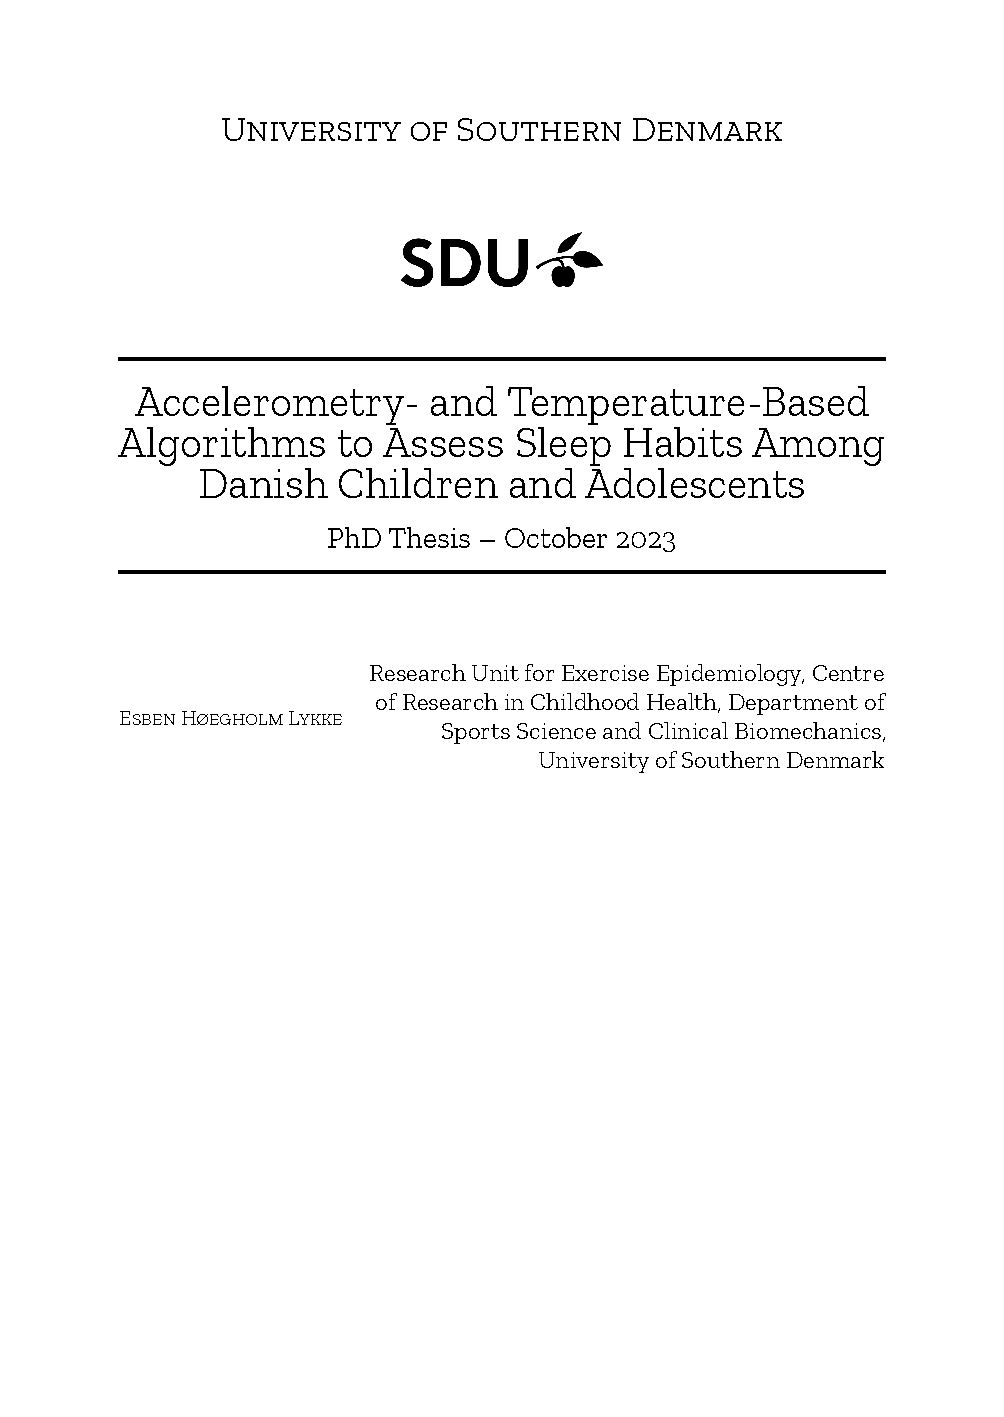
\includepdf[pages=-]{titlepage.pdf}

\newpage

\textsf{\textbf{\Large{Supervisor}}}

\vspace*{\baselineskip}

Associate Professor Jan Christian Brønd, PhD

Research Unit for Exercise Epedimiology, Centre of Research in Childhood Health, Department of Sports Science and Clinical Biomechanics, University of Southern Denmark, Odense, Denmark

\vspace{2cm}

\textsf{\textbf{\Large{Assessment Committee}}}

\vspace*{\baselineskip}

\textbf{Chair}

Professor WSR Jasper Schiperijn, PhD

Research Unit of Active Living, Danish centre for motivation and behaviour science, Playground Research, Department of Sports Science and Clinical Biomechanics, University of Southern Denmark, 5230 Odense, Denmark

\textbf{Opponents}

Associate Professor Samuel Emil Schmidt, PhD

Department of Health Science and Technology, Aalborg University, Denmark

Associate Professor Alex Rowlands, PhD

Diabetes Research Centre, NIHR Leicester Biomedical Research Centre - Lifestyle Theme, University of Leicester, United Kingdom

\vspace{2cm}

\textsf{\textbf{\Large{Funding}}}

\vspace*{\baselineskip}

The research presented in this thesis was generously funded by TrygFonden, under grant numbers ID 130081 and 115606, and by the European Research Council, under grant number 716657. Additional support was provided by a one-year scholarship from the Faculty of Health Sciences.

\newpage

%----------------------------------------------
  %   Preface
%----------------------------------------------
  
\textsf{\textbf{\Large{Preface}}}

\vspace*{\baselineskip}

The journey of my PhD has been a fulfilling expedition, layered with explorations, discoveries, struggles, and growth. This endeavor was fueled by my interest in understanding the objective measurements of physical behavior and sleep. During my Masters, I found myself increasingly engrossed in these domains.

My subsequent role as a research assistant at Aarhus University opened another dimension of learning for me. The works of my peers, employing machine learning and advanced statistics on accelerometer data, intrigued me. It was as if I found the nexus of my research interests, a perfect alignment that seamlessly fused my curiosities and passions.

One of the most significant hurdles was my limited experience with programming and machine learning, which proved to be a steep learning curve. However, through persistence, I slowly developed the necessary skills to analyze and interpret my data effectively. Another major setback was the failed data collection for my third paper. I spent months visiting families, mounting an ambulatory PSG device on children before bedtime, and facing the harsh reality of dealing with poor data quality.

This thesis brings together my explorations and findings across three papers that carry a consistent emphasis on improving and validating methods to leverage accelerometer data for studying human behaviors. The common thread across these papers is the application of innovative methods, particularly machine learning techniques, to enhance the utility, reliability, and accuracy of free-living accelerometer data for monitoring human sleep and physical activity. The work presented here constitutes a substantial contribution to the field of sleep and physical activity research, particularly in the context of large-scale studies.

Two of these papers have already found their place in peer-reviewed scientific journals, and the third is under review. All of these works are included as appendices to this thesis, and their content has been weaved into the fabric of this thesis.

As I look back at my journey through the PhD program, I am grateful for this opportunity to delve deep into a subject that I am passionate about and to contribute to a field that is evolving rapidly. This experience has instilled in me a sense of tenacity and patience, qualities that I have come to value deeply. I learned that even the most frustrating problems have solutions, and the path to those solutions often leads to personal growth and novel insights.

As I stand on the precipice of my future, I am filled with a sense of anticipation and excitement for the possibilities that lie ahead. I am eager to explore new horizons, to encounter new challenges, and to continue growing as a researcher and as an individual. However, wherever I go and whatever I do, I will carry with me the memories, experiences, and lessons from this incredible journey.

These years have shaped me in ways I could never have imagined at the outset, and for that, I am profoundly grateful. As I close this chapter of my life, I do so with a sense of accomplishment and a promise of continued exploration and discovery in my field. After all, every ending is but a new beginning, and I look forward to the adventures that await.

\newpage

%----------------------------------------------
  %   Acknowledgement
%----------------------------------------------
  
\textsf{\textbf{\Large{Acknowledgment}}}

\vspace*{\baselineskip}

Throughout this journey, there have been several people who have influenced, inspired, and supported me. My Main Supervisor, Jan Christian Brønd, deserves special mention for his guidance and patience. His commitment to nurturing my development as a researcher and lecturer has been instrumental. Our collaborative dialogues, be it at the office or during examinations, have been pivotal in my growth. I also extend my sincere gratitude to my co-supervisors [insert name 2] and [insert name 3], and my colleague [insert name 4], who have always provided invaluable insights and perspectives.

Amidst all the academic pursuits, my family remained the cornerstone of my journey. My wife, the bedrock of our family, kept our home running smoothly and offered endless support and curiosity about my work. The joy and love from my four children were my constant sources of motivation and inspiration.

The PhD journey has taught me the importance of rigour and attention to detail. My approach to work has been permanently shaped by my experience as a researcher. The discipline and precision that is required in research has translated into my everyday life, impacting my approach to problem-solving, decision-making, and even communication. It's impressive how research is not merely a vocation but a lens through which we view the world.

There were also moments of immense joy and satisfaction, like finally solving a complex analytical problem, having my work accepted for publication, or simply receiving positive feedback from a student or a colleague. Those moments fueled my motivation and reminded me of the importance and impact of my work.

One of the most rewarding aspects of this journey was the opportunity to be part of an international recognized and experienced research group. This gave me the chance to work with and learn from some of the most talented people in my field, to discuss ideas and collaborate on projects, and to be part of a collective effort to advance knowledge and understanding in our field.

In retrospect, this PhD journey has been much more than a professional pursuit. It has been a personal voyage of self-discovery and growth. Through the highs and lows, the victories and setbacks, the late nights and early mornings, I've discovered a resilience in myself that I hadn't known before. I found that I could rise to challenges, learn from failures, and continue to strive for excellence, no matter the odds.

In closing, I wish to express my deep gratitude for all those who have supported me throughout this journey - my supervisors, colleagues, friends, and family. Their faith in my abilities and their constant encouragement have been my pillars of strength. I hope that the work presented in this thesis reflects the depth of my dedication and the extent of my learning journey.

\newpage

\textsf{\textbf{\Large{Included Papers}}}

\vspace{2cm}

\begin{center}

Paper I

\textsf{Manual Annotation of Time in Bed Using Free-Living Recordings of Accelerometry Data}

published in \href{https://doi.org/10.3390/s21248442}{Sensors}

\vspace{2cm}
Paper II

\textsf{Generalizability and Performance of Methods to Detect Non‑Wear with Free‑Living Accelerometer Recordings}

published in \href{https://doi.org/10.1038/s41598-023-29666-x}{Scientific Reports}

\vspace{2cm}
Paper III 

\textsf{Improving Sleep Quality Estimation: A Comparative Study of Machine Learning and Deep Learning Techniques Utilizing Free-Living Accelerometer Data from Thigh-Worn Devices and EEG-Based Sleep Tracking}

Submitted to \href{https://www.nature.com/npjdigitalmed/}{npj Digital Medicine}

\end{center}

\newpage\renewcommand*\contentsname{Table of contents}
{
\hypersetup{linkcolor=}
\setcounter{tocdepth}{3}
\tableofcontents
}
\aftertocpagenum

\newpage

\hypertarget{english-summary}{%
\section{English Summary}\label{english-summary}}

bla

\newpage

\hypertarget{danish-summary}{%
\section{Danish Summary}\label{danish-summary}}

bla

\newpage

\hypertarget{introduction}{%
\section{Introduction}\label{introduction}}

\hypertarget{outline-of-introduction-section}{%
\subsection{Outline of Introduction
Section}\label{outline-of-introduction-section}}

\begin{itemize}
\tightlist
\item
  The importance of sleep and physical activity tracking in health
  research.
\end{itemize}

Physical behaviors throughout a day encompass a range of activities,
including sleep, physical activity (PA), and sedentary behavior.
Numerous studies over the past decade have underscored the health
benefits of optimal sleep, high PA levels, especially
moderate-to-vigorous physical activity
(MVPA)\textsuperscript{\protect\hyperlink{ref-kraus_physical_2019}{1},\protect\hyperlink{ref-lee_effect_2012}{2}},
minimal sedentary
periods\textsuperscript{\protect\hyperlink{ref-wilmot_sedentary_2012}{3}},
and adequate
sleep\textsuperscript{\protect\hyperlink{ref-cappuccio_sleep_2010}{4}}.
This robust evidence has informed public
guidelines\textsuperscript{\protect\hyperlink{ref-borodulin_physical_2023}{\textbf{borodulin\_physical\_2023?}}},
such as the American recommendation of 150 minutes of MVPA per
week\textsuperscript{\protect\hyperlink{ref-kl_physical_2018}{5}}, and
the Danish guideline suggesting 30 minutes of MVPA daily for
adults\textsuperscript{\protect\hyperlink{ref-el-zine_fysisk_nodate-1}{6}}
and 60 minutes for
children\textsuperscript{\protect\hyperlink{ref-el-zine_fysisk_nodate}{7}}.

The integration of sleep and physical activity tracking in health
research is paramount for a comprehensive understanding of individual
well-being. Over the years, the significance of both sleep and physical
activity in maintaining optimal health has been increasingly
acknowledged\textsuperscript{\protect\hyperlink{ref-kraus_physical_2019}{1},\protect\hyperlink{ref-lee_effect_2012}{2},\protect\hyperlink{ref-liguori_evolving_2023}{8}}.
These elements are foundational to our well-being, influencing a
spectrum of health aspects from mental
health\textsuperscript{\protect\hyperlink{ref-biddle_physical_2011}{9}}
to physical
fitness\textsuperscript{\protect\hyperlink{ref-warburton_health_2017}{10}},
and even disease
prevention\textsuperscript{\protect\hyperlink{ref-strath_guide_2013}{11},\protect\hyperlink{ref-arem_leisure_2015}{12}}.

With the advent of wearable technology and advanced tracking systems,
researchers now possess tools that allow for an in-depth exploration of
the intricate relationship between sleep, physical activity, and overall
health\textsuperscript{\protect\hyperlink{ref-rollo_whole_2020}{13}}.
Traditional health assessments might have primarily focused on diet,
weight, or blood pressure. However, by incorporating data on sleep and
physical activity, we can achieve a more holistic understanding of
health. For instance, sleep deprivation is associated with a range of
health issues, from weight gain and decreased immune function to an
increased risk of chronic diseases like diabetes and cardiovascular
disease\textsuperscript{\protect\hyperlink{ref-warburton_health_2017}{10}}.

Building on this, the ability to monitor sleep and physical activity has
revolutionized personalized health interventions. For example, if data
reveals interrupted sleep patterns, interventions can be customized to
address these specific issues. Similarly, if someone isn't achieving
their physical activity targets, strategies can be formulated to boost
their activity levels, potentially enhancing health
outcomes\textsuperscript{\protect\hyperlink{ref-rosenberger_24-hour_2019}{14}}.
Furthermore, tracking these patterns provides researchers with insights
into the mechanisms of various diseases and health conditions. Early
detection of conditions like sleep apnea, characterized by intermittent
breathing pauses during sleep, can lead to timely management, preventing
a cascade of health
complications\textsuperscript{\protect\hyperlink{ref-cappuccio_sleep_2010}{4}}.
For patients undergoing treatments, such as those with depression who
often face sleep disturbances, tracking becomes vital. It allows
healthcare providers to assess the effectiveness of interventions,
whether they're antidepressant medications or other therapeutic
strategies\textsuperscript{\protect\hyperlink{ref-paruthi_consensus_2016}{15}}.

In today's medical landscape, there's a pronounced focus on preventive
healthcare. The principle is clear: it's better to prevent diseases than
to treat them after they manifest. Regular tracking of sleep and
physical activity can act as an early warning system, signaling
potential health risks before they develop into severe conditions. For
instance, consistent inactivity can heighten risks related to obesity,
heart disease, and other chronic
ailments\textsuperscript{\protect\hyperlink{ref-tremblay_sedentary_2017}{16}}.
Early detection through tracking can pave the way for timely
interventions and preventive
actions\textsuperscript{\protect\hyperlink{ref-liguori_evolving_2023}{8}}.

\begin{itemize}
\tightlist
\item
  measurement of physical activity and sleep
\item
  subjective methods
\item
  objective methods
\end{itemize}

\hypertarget{measurement-of-physical-activity-and-sleep}{%
\subsection{Measurement of Physical Activity and
Sleep}\label{measurement-of-physical-activity-and-sleep}}

Physical activity and sleep are integral components of human behavior.
Physical activity is characterized by multiple dimensions such as
frequency, duration, intensity, and domains, making it challenging to
measure all its aspects (21). Similarly, sleep is essential for health,
and its accurate monitoring in terms of duration, quality, architecture,
and circadian patterns is crucial. Various techniques are available to
quantify both PA and sleep, broadly grouped into subjective and
objective methods.

\hypertarget{subjective-methods}{%
\subsubsection{Subjective Methods}\label{subjective-methods}}

Physical Activity Questionnaires and Diaries/Logs

In epidemiological studies, self-report methods, including PA
questionnaires and diaries, have been primary tools due to their low
cost, ease of use, and ability to capture the type and context of
PA(25). Despite their advantages, these methods can be prone to biases,
including reporting bias and misinterpretation, and may not always be
reliable(25).

Sleep Questionnaires and Diaries

Subjective sleep quality can be assessed using tools like the Pittsburgh
Sleep Quality Index, reflecting one's satisfaction with sleep over a
specified period, such as a month(78). While they are practical and
cost-effective, self-report sleep assessments can overestimate sleep
duration and may not capture all nuances of sleep quality(79). Sleep
diaries, often regarded as the ``gold standard'' for subjective sleep
assessment, provide daily insights but are dependent on memory and
participant adherence(82).

\hypertarget{objective-methods}{%
\subsubsection{Objective Methods}\label{objective-methods}}

Direct Observation and Polysomnography (PSG)

Direct observation allows researchers to record an individual's PA and
sleep behaviors, capturing intricate details like frequency, duration,
and intensity(21). PSG, on the other hand, is the gold standard for
sleep measurement, monitoring various physiological aspects in a
controlled setting(78). Both methods, while comprehensive, can be costly
and labor-intensive.

Doubly Labelled Water Method

This method provides an estimate of total energy expenditure over
several days and is a gold standard for PA(25). It's a powerful tool but
comes with high costs and doesn't provide granular details on PA
dimensions(26).

Physiological Recordings

Heart rate (HR) recordings can be used to estimate PA intensity,
assuming a linear relationship between HR and PA intensity(27). While
relatively cost-effective, various external factors can influence HR,
making it less accurate for certain activities(27).

Device-based Methods: Pedometers, Accelerometers, and Actigraphy

Pedometers are simple devices that count steps and can provide
additional metrics like distance traveled and calories burned(21).
Accelerometers, such as GENEActiv and ActiGraph, offer detailed
recordings of raw triaxial linear acceleration data, capturing a wide
range of PA and sleep data(28). Wrist actigraphy, commonly used in sleep
research, measures wrist movements to assess sleep or waking state(85).
These devices are convenient and non-intrusive, but their data might
vary due to different technical characteristics, making direct
comparisons challenging(33).

\hypertarget{sleep-assessment-with-accelerometry}{%
\subsubsection{Sleep Assessment with
Accelerometry}\label{sleep-assessment-with-accelerometry}}

Wrist-worn accelerometers have become increasingly popular for PA
assessment. They have been developed separately from clinical wrist
actigraphy but offer the potential for dual PA and sleep data
collection(90). New algorithms, like the GGIR-package in R, combine
24-hour activity data, but they often require a sleep log for
accuracy(92). Some algorithms can detect sleep periods even without
sleep diaries, but their validation remains limited(93).

\begin{itemize}
\tightlist
\item
  Gold standards
\item
  Traditional methods and their limitations
\item
  polysomnography
\item
  self-reported diaries
\item
  The emergence and potential of wearable accelerometers and some kind
  segway to machine learning models in this field.
\end{itemize}

Some of these limitations can be addressed with 24-hour
accelerometer-based protocols, especially those worn on the
wrist\textsuperscript{\protect\hyperlink{ref-rosenberger_24-hour_2019}{14}}.
Wrist accelerometers are small, non-invasive,
waterproof\textsuperscript{\protect\hyperlink{ref-welk_reliability_2004}{17}},
allowing for continuous, 24-hour wear with minimal disruption to the
wearer, and permit uninterrupted activity measurement throughout the
day, thereby tracking and analyzing daily changes in PA and sleep
behaviors. Furthermore, the latest accelerometers supply raw
acceleration data that can be processed using open-source analytical
techniques to produce estimates of sleep, sedentary behavior, and
PA\textsuperscript{\protect\hyperlink{ref-migueles_comparability_2019}{18}}.
Simultaneous measurement of physical behaviors, particularly feasible
with wrist accelerometry, can offer a better comprehension of the
influence of these behaviors on health indicators and their
interrelationships. This data could be critical in shaping future health
recommendations or interventions.

\begin{itemize}
\tightlist
\item
  Supervised learning and annotation of data sources
\end{itemize}

Machine learning stands at the crossroads of statistics and computer
science. It embodies the principles of discerning patterns and
relationships from data, a foundational tenet of statistics, while also
leveraging the power of efficient computing algorithms, a core concept
in computer
science\textsuperscript{\protect\hyperlink{ref-hastie01statisticallearning}{19}}.
With the surge in data scale, encompassing billions or even trillions of
data points, this synergy becomes essential to navigate the intricate
landscape of data analysis.

One of the primary branches of machine learning is supervised learning.
Its primary objective is to predict known outputs based on inputs.
Real-world applications of supervised learning span across various
domains. For instance, in machine learning competitions, challenges
often include tasks such as handwriting recognition, image
classification (e.g., discerning between a cat and a dog), and document
categorization (e.g., differentiating between a clinical trial on heart
failure and a financial report). These tasks aim to emulate or even
surpass human capabilities in specific areas. Supervised learning
essentially revolves around two core concepts: classification
(categorizing data into predefined groups) and prediction (estimating
unknown parameters).

Delving deeper into its applications, consider the realm of physical
activity and sleep research. Here, supervised learning plays a pivotal
role. For instance, algorithms can automatically classify activity
levels---from sedentary to vigorous---using data from accelerometers.
Similarly, in sleep studies, such algorithms can discern between various
sleep stages like light sleep or REM, using accelerometer or actigraphy
data. While these machines emulate human analysts, their capabilities
can extend beyond, unveiling insights or patterns not immediately
visible to human researchers. A predictive model, for example, might
forecast the risk of metabolic syndrome based on sedentary time patterns
or predict sleep disorders from sleep pattern variations. (REFS PÅ HELE
AFSNITTET)

The utilization of machine learning to decipher sleep and physical
activity from accelerometry data is gaining traction. Its capability to
model intricate non-linear relationships is unparalleled compared to
traditional statistical methods like linear
regression\textsuperscript{\protect\hyperlink{ref-fiorillo_automated_2019}{20}}.
Yet, the success of supervised learning hinges on abundant and
accurately annotated data for ensuring both precision and
applicability\textsuperscript{\protect\hyperlink{ref-van_der_ploeg_modern_2014}{21}}.

The significance of sleep, especially for children's health and
development, is
well-established\textsuperscript{\protect\hyperlink{ref-chaput_systematic_2017}{22}--\protect\hyperlink{ref-st-onge_sleep_2016}{24}}.
Healthy sleep encompasses several factors like duration, timing, and
quality\textsuperscript{\protect\hyperlink{ref-gruber_position_2014}{25}}.
Yet, the potential of advanced machine learning in evaluating sleep
using accelerometer data is still largely
untapped\textsuperscript{\protect\hyperlink{ref-haghayegh_application_2020}{26}}.

Despite the supremacy of Polysomnography (PSG) as the gold standard for
objective sleep analysis, its high costs, and intrusive nature
underscore the value of accelerometry---a less invasive and more
cost-effective
alternative\textsuperscript{\protect\hyperlink{ref-vaughn_technical_2008}{27}}.
Recent endeavors in this domain include PSG-assessed sleep-wake
classification using wrist-worn accelerometers. For example,
Sundararajan et
al.\textsuperscript{\protect\hyperlink{ref-sundararajan_sleep_2021}{28}}
leveraged a random forest machine learning algorithm, achieving
commendable results. Yet, issues like high false discovery rates point
to challenges such as limited subject variation.

To address these challenges, there's a clear imperative to diversify the
sample base and extend recording durations. While accelerometry has its
limitations, its feasibility for prolonged, out-of-lab recordings makes
it
invaluable\textsuperscript{\protect\hyperlink{ref-van_de_water_objective_2011}{29}}.
Given these dynamics, the focus should lean towards sleep timing
algorithms rather than sleep staging.

A crucial aspect of deciphering sleep/wake cycles from accelerometry
data is the annotation of time in bed, which, although not indicative of
actual sleep duration, provides crucial insights. Such annotations can
stem from individual sleep diaries, EEG-based
recordings\textsuperscript{\protect\hyperlink{ref-younes_staging_2016}{30}},
or systems capturing tracheal
sounds\textsuperscript{\protect\hyperlink{ref-dafna_sleep-wake_2015}{31},\protect\hyperlink{ref-montazeri_ghahjaverestan_sleepwakefulness_2020}{32}}.
Given its practicality, accelerometry continues to be a staple in sleep
research, echoing its immense potential and
adaptability\textsuperscript{\protect\hyperlink{ref-hees_novel_2015}{33}--\protect\hyperlink{ref-barouni_ambulatory_2020}{36}}.

\begin{itemize}
\tightlist
\item
  Nonwear
\item
  Sleep
\end{itemize}

\hypertarget{scope-and-relevance}{%
\paragraph{Scope and Relevance}\label{scope-and-relevance}}

\begin{itemize}
\tightlist
\item
  The need for cost-effective, reliable, and practical alternatives for
  large-scale studies.
\item
  The potential of free-living accelerometers, and why they are a
  compelling subject of study.
\end{itemize}

\hypertarget{existing-challenges}{%
\paragraph{Existing Challenges}\label{existing-challenges}}

\begin{itemize}
\tightlist
\item
  Discuss the challenges with existing methods, such as identifying
  non-wear time, annotating in-bed periods, and classifying awake
  periods during in-bed time.
\item
  Address the lack of exploration of certain sensor locations, like the
  thigh.
\end{itemize}

\hypertarget{thesis-goals-and-objectives}{%
\paragraph{Thesis Goals and
Objectives}\label{thesis-goals-and-objectives}}

\begin{itemize}
\tightlist
\item
  Clearly state the aim and objectives of your thesis.
\item
  Explain how your thesis will address the identified challenges,
  including improving the manual annotation of in-bed periods, enhancing
  non-wear detection, and estimating sleep quality metrics.
\end{itemize}

\hypertarget{overview-of-the-papers}{%
\paragraph{Overview of the Papers}\label{overview-of-the-papers}}

\begin{itemize}
\item
  Briefly introduce each paper, highlighting the key research question,
  methods, and findings.
\item
  Explain how each paper contributes to your thesis goals and
  objectives.
\end{itemize}

\hypertarget{motivation-for-the-research}{%
\subsubsection{Motivation for the
Research}\label{motivation-for-the-research}}

\hypertarget{the-need-for-improved-annotation-techniques}{%
\paragraph{The Need for Improved Annotation
Techniques}\label{the-need-for-improved-annotation-techniques}}

\begin{itemize}
\tightlist
\item
  Importance of accurate annotation in accelerometer data analysis.
\item
  A brief discussion of the first paper's findings and implications.
\end{itemize}

\hypertarget{improving-non-wear-detection}{%
\paragraph{Improving Non-Wear
Detection}\label{improving-non-wear-detection}}

\begin{itemize}
\tightlist
\item
  Explain the implications of undetected non-wear time on data quality.
\item
  Highlight the findings of your second paper and its relevance.
\end{itemize}

\hypertarget{advancing-sleep-quality-estimation}{%
\paragraph{Advancing Sleep Quality
Estimation}\label{advancing-sleep-quality-estimation}}

\begin{itemize}
\tightlist
\item
  Discuss the impact of sleep quality estimation on understanding human
  sleep behavior.
\item
  Briefly describe the conclusions of your third paper.
\end{itemize}

\hypertarget{methodological-approaches}{%
\subsubsection{Methodological
Approaches}\label{methodological-approaches}}

\begin{itemize}
\item
  Give a brief overview of the methods used across all three studies,
  such as the use of machine learning models, deep learning techniques,
  manual annotation, and decision tree models.
\item
  Explain how these methods address the research objectives and the
  challenges identified earlier.
\end{itemize}

\hypertarget{thesis-structure}{%
\subsubsection{Thesis Structure}\label{thesis-structure}}

Provide an outline of the subsequent chapters of your thesis.

\newpage

\hypertarget{manual-annotation-of-time-in-bed-using-free-living-recordings-of-accelerometry-data}{%
\section{Manual Annotation of Time in Bed Using Free-Living Recordings
of Accelerometry
Data}\label{manual-annotation-of-time-in-bed-using-free-living-recordings-of-accelerometry-data}}

This segment of the thesis encompasses the methods, results, and
discussion for Paper I. The study underscores the importance of
effective machine learning algorithms for sleep/wake cycles, which
ideally necessitate correct data annotations over a span of 7-10 days.
Although sleep diaries or EEG recordings can annotate `time in bed',
many researches predominantly rely on accelerometry. This emphasizes the
imperative for enhanced annotation techniques and their validity. Our
objective is to introduce a manual annotation method, gauge its
precision, and determine its consistency. Some of the details presented
here were previously mentioned in the published version of Paper
I\textsuperscript{\protect\hyperlink{ref-skovgaard_manual_2021}{37}}.

\hypertarget{methods}{%
\subsection{Methods}\label{methods}}

\hypertarget{study-population}{%
\subsubsection{Study Population}\label{study-population}}

The data for this study was sourced from the SCREENS pilot trial
(www.clinicaltrials.gov, NCT03788525), a two-arm parallel-group
cluster-randomized trial with two intervention groups, conducted between
October 2018 and March
2019\textsuperscript{\protect\hyperlink{ref-rasmussen_feasibility_2021}{38},\protect\hyperlink{ref-rasmussen_short-term_2020}{39}}.
There was no control group in this trial.

Families from the Middelfart municipality in Denmark were approached for
participation if they had a child aged between 6 to 10 years living with
them, out of a total of 1686 families. To qualify, the parent's screen
media usage had to exceed the median of 2.7 hours per day, based on
survey responses from 394 respondents. Additionally, all children in the
household needed to be older than 3.9 years to ensure that sleep
measurements weren't disrupted by the nocturnal awakenings typical of
infants or toddlers. For a comprehensive list of inclusion and exclusion
criteria, refer to Pedersen et
al.\textsuperscript{\protect\hyperlink{ref-pedersen_self-administered_2021}{40}}.

The study ultimately included data from 14 children and 19 adults. These
participants weren't advised to alter their sleep or bedtime routines
for the interventions. While the study focused on nightly sleep time as
recorded by the EEG-based sleep staging system, any napping behavior of
the participants was deemed irrelevant.

All data collection procedures were reported to the local data
protection department, SDU RIO (ID: 10.391), in compliance with the
Danish Data Protection Agency's regulations.

\hypertarget{actigraphy}{%
\subsubsection{Actigraphy}\label{actigraphy}}

Both adults and children participated in 24-hour accelerometry
recordings using two triaxial accelerometers, Axivity AX3 (Axivity Ltd.,
Newcastle upon Tyne, UK). The Axivity AX3 is a compact device, measuring
23 mm × 32.5 mm × 7.6 mm and weighing just 11 g. It was set with a
sensitivity of ±8 g and a sampling frequency of 50 Hz.

Participants wore the accelerometers at two specific anatomical
locations. The first was positioned on the right hip, secured in a
pocket attached to a belt around the waist, ensuring the USB connector
faced outward from the body's right side. The second accelerometer was
placed midway between the hip and knee on the right thigh, housed in a
pocket on a belt, with the USB connector also facing away from the body.

For both the baseline and follow-up, the devices were worn for a
duration of one week (seven consecutive days). This duration aligns with
the recommended number of days to reliably gauge habitual physical
activity\textsuperscript{\protect\hyperlink{ref-jaeschke_variability_2018}{41}}.

\hypertarget{zmachine-insight-sleep-assessments}{%
\subsubsection{Zmachine® Insight+ Sleep
Assessments}\label{zmachine-insight-sleep-assessments}}

Both adults and children were assessed for their sleep patterns using
the Zmachine® (ZM) Insight+ model DT-200 (General Sleep Corporation,
Cleveland, OH, USA), Firmware version 5.1.0. This assessment was
concurrent with the accelerometer recordings. At the baseline, the sleep
assessment spanned 3--4 nights, while during the follow-up, it was
conducted over 3 nights.

The ZM device operates by measuring sleep through a single-channel EEG,
specifically from the differential mastoid (A1--A2) EEG location,
evaluated on a 30-second epoch basis. Designed for use in everyday
settings, the ZM provides an objective measurement of various sleep
parameters, including sleep duration, sleep stage classification, and
latency to different sleep stages.

The ZM's algorithm has been benchmarked against polysomnography (PSG) in
laboratory settings for both adults with and without chronic sleep
issues\textsuperscript{\protect\hyperlink{ref-wang_evaluation_2015}{42},\protect\hyperlink{ref-kaplan_performance_2014}{43}}.
Our findings indicate that the ZM is effectively applicable to both
children and adults for multi-day measurements in real-world
settings\textsuperscript{\protect\hyperlink{ref-hees_novel_2015}{33}}.
Notably, the device showcased a high accuracy in distinguishing between
sleep and wakefulness, with sensitivity, specificity, positive
predictive value, and negative predictive values being 95.5\%, 92.5\%,
98\%, and 84.2\%,
respectively\textsuperscript{\protect\hyperlink{ref-kaplan_performance_2014}{43}}.

For the assessment, three electrodes (Ambu A/S, Ballerup, Denmark, type:
N-00-S/25) are positioned on the mastoids (for signal) and the nape (as
ground). About half an hour before their intended sleep time,
participants' skin areas are cleaned with alcohol swabs, after which the
electrodes are affixed. An EEG cable connects these electrodes to the ZM
device. A preliminary sensor check ensures all electrodes are correctly
mounted; any issues are promptly addressed by replacing the problematic
electrodes. Additionally, participants, or parents on behalf of their
children, recorded their sleep and wake times daily in a dedicated
diary.

\hypertarget{audacity}{%
\subsubsection{Audacity}\label{audacity}}

Audacity®️ is a distinguished free audio editing
software\textsuperscript{\protect\hyperlink{ref-audacity}{44}}. The
genesis of Audacity can be traced back to the fall of 1999, when it
emerged as an innovative project led by Dominic Mazzoni and Roger
Dannenberg at Carnegie Mellon University. By May 2000, it was unveiled
to the world as an open-source audio editor. Since its inception,
Audacity has undergone significant evolution. The software, developed
collaboratively by the community, now boasts of hundreds of unique
features, offers complete support for professional-grade 24-bit and
32-bit audio, has a comprehensive manual available in multiple
languages, and has witnessed distribution in the millions. Today, a
dedicated team of volunteers from various corners of the globe continues
to maintain and enhance Audacity. It is disseminated under the GNU
General Public License, granting everyone the freedom to utilize the
software for personal, educational, or commercial endeavors.

In the realm of accelerometer data analysis, Audacity stands out. It
furnishes researchers with the capability to meticulously scrutinize
high-resolution raw accelerometer data with unparalleled precision.
Users can quickly zoom in to delve deeper into specific segments of the
recording, like certain patterns around bedtime, or zoom out for a
broader perspective, such as data spanning a week. Furthermore,
Audacity's sophisticated labeling function is pivotal for annotating the
accelerometry data. Any generated labels can be preserved in an
individual file and later integrated into machine learning algorithms.
This level of detailed manual inspection of high-resolution
accelerometer data offered by Audacity is, based on our knowledge,
unparalleled by any other software.

Within the Audacity interface, there's the possibility of amalgamating
over 100 channels of data. This aids in the merging of distinct signal
features derived from acceleration. The integration of multiple signal
features is intriguing as it might enhance the visual comprehension and
classification of inherent behaviors. Nevertheless, an excessive
conglomeration of signal features might obscure the precise
identification of targeted behaviors. For our study, we incorporated a
total of seven distinct signal features. The criteria for classifying
``lying'' in the first feature are explicit: if the inclination of the
hip accelerometer surpasses 65 degrees and the thigh accelerometer
simultaneously identifies as ``sitting'' based on Skotte et al.'s
activity type classification
algorithm\textsuperscript{\protect\hyperlink{ref-skotte_detection_2014}{45}}.
The other signal features, barring ``time'', are directly procured from
Skotte et al.'s algorithm. These features, delineated in Table 1,
concern the longitudinal axis of the body. Data derived from
accelerometry undergoes processing using a window length of two seconds
(60 samples) and has a 50\% overlap (30 samples), ensuring a resolution
of one second. The methodologies from Skotte et al.~and those generating
the first feature rely exclusively on the accelerometer's
inclination(s). Hence, while they can determine time in bed and
participant's posture, they aren't precise indicators for pinpointing
exact in-bed and out-of-bed moments.

To provide a visual perspective, Figure~\ref{fig-screen_full} and
Figure~\ref{fig-screen_night} depict the Audacity interface displaying
all seven signal features as cataloged in
Table~\ref{tbl-man_signal_features}. Figure~\ref{fig-screen_full} offers
a glimpse of a week's data, whereas Figure~\ref{fig-screen_night} zooms
into an approximate 24-hour span, showcasing a single annotated night.

\newpage

\begingroup

\footnotesize

\hypertarget{tbl-man_signal_features}{}
\begin{longtable}{lll}
\caption{\label{tbl-man_signal_features}Summary of the specific signal features utilized in Audacity for the
accurate detection and analysis of in-bed periods. }\tabularnewline

\toprule
Name & Description & Values \\ 
\midrule
Lying & Classification based on thigh and back & 1: lying, -1: not lying \\ 
Activity & Activity type classification & 1: Standing, moving, 0: Sitting, -1: Other \\ 
Time & Time categorized into four-hour windows & Time categorized throughout 24 h cycle \\ 
Thigh-SDacc & Thigh longitudinal acceleration SD & -1: No movement \\ 
Thigh-Inclination & Thigh device inclination angle & Range: −180 to 180 degrees \\ 
Hip-SDacc & Hip longitudinal acceleration SD & -1: No movement \\ 
Hip-Inclination & Hip device inclination angle & Range: −180 to 180 degrees \\ 
\bottomrule
\end{longtable}

\endgroup

\begin{figure}

{\centering \includegraphics{figures/audacity_full_view.png}

}

\caption{\label{fig-screen_full}Screenshot of the Audacity interface
showing the seven horizontal panels representing the included signal
features. See Table~\ref{tbl-man_signal_features} for a detailed
description of the features.}

\end{figure}

\begin{figure}

{\centering 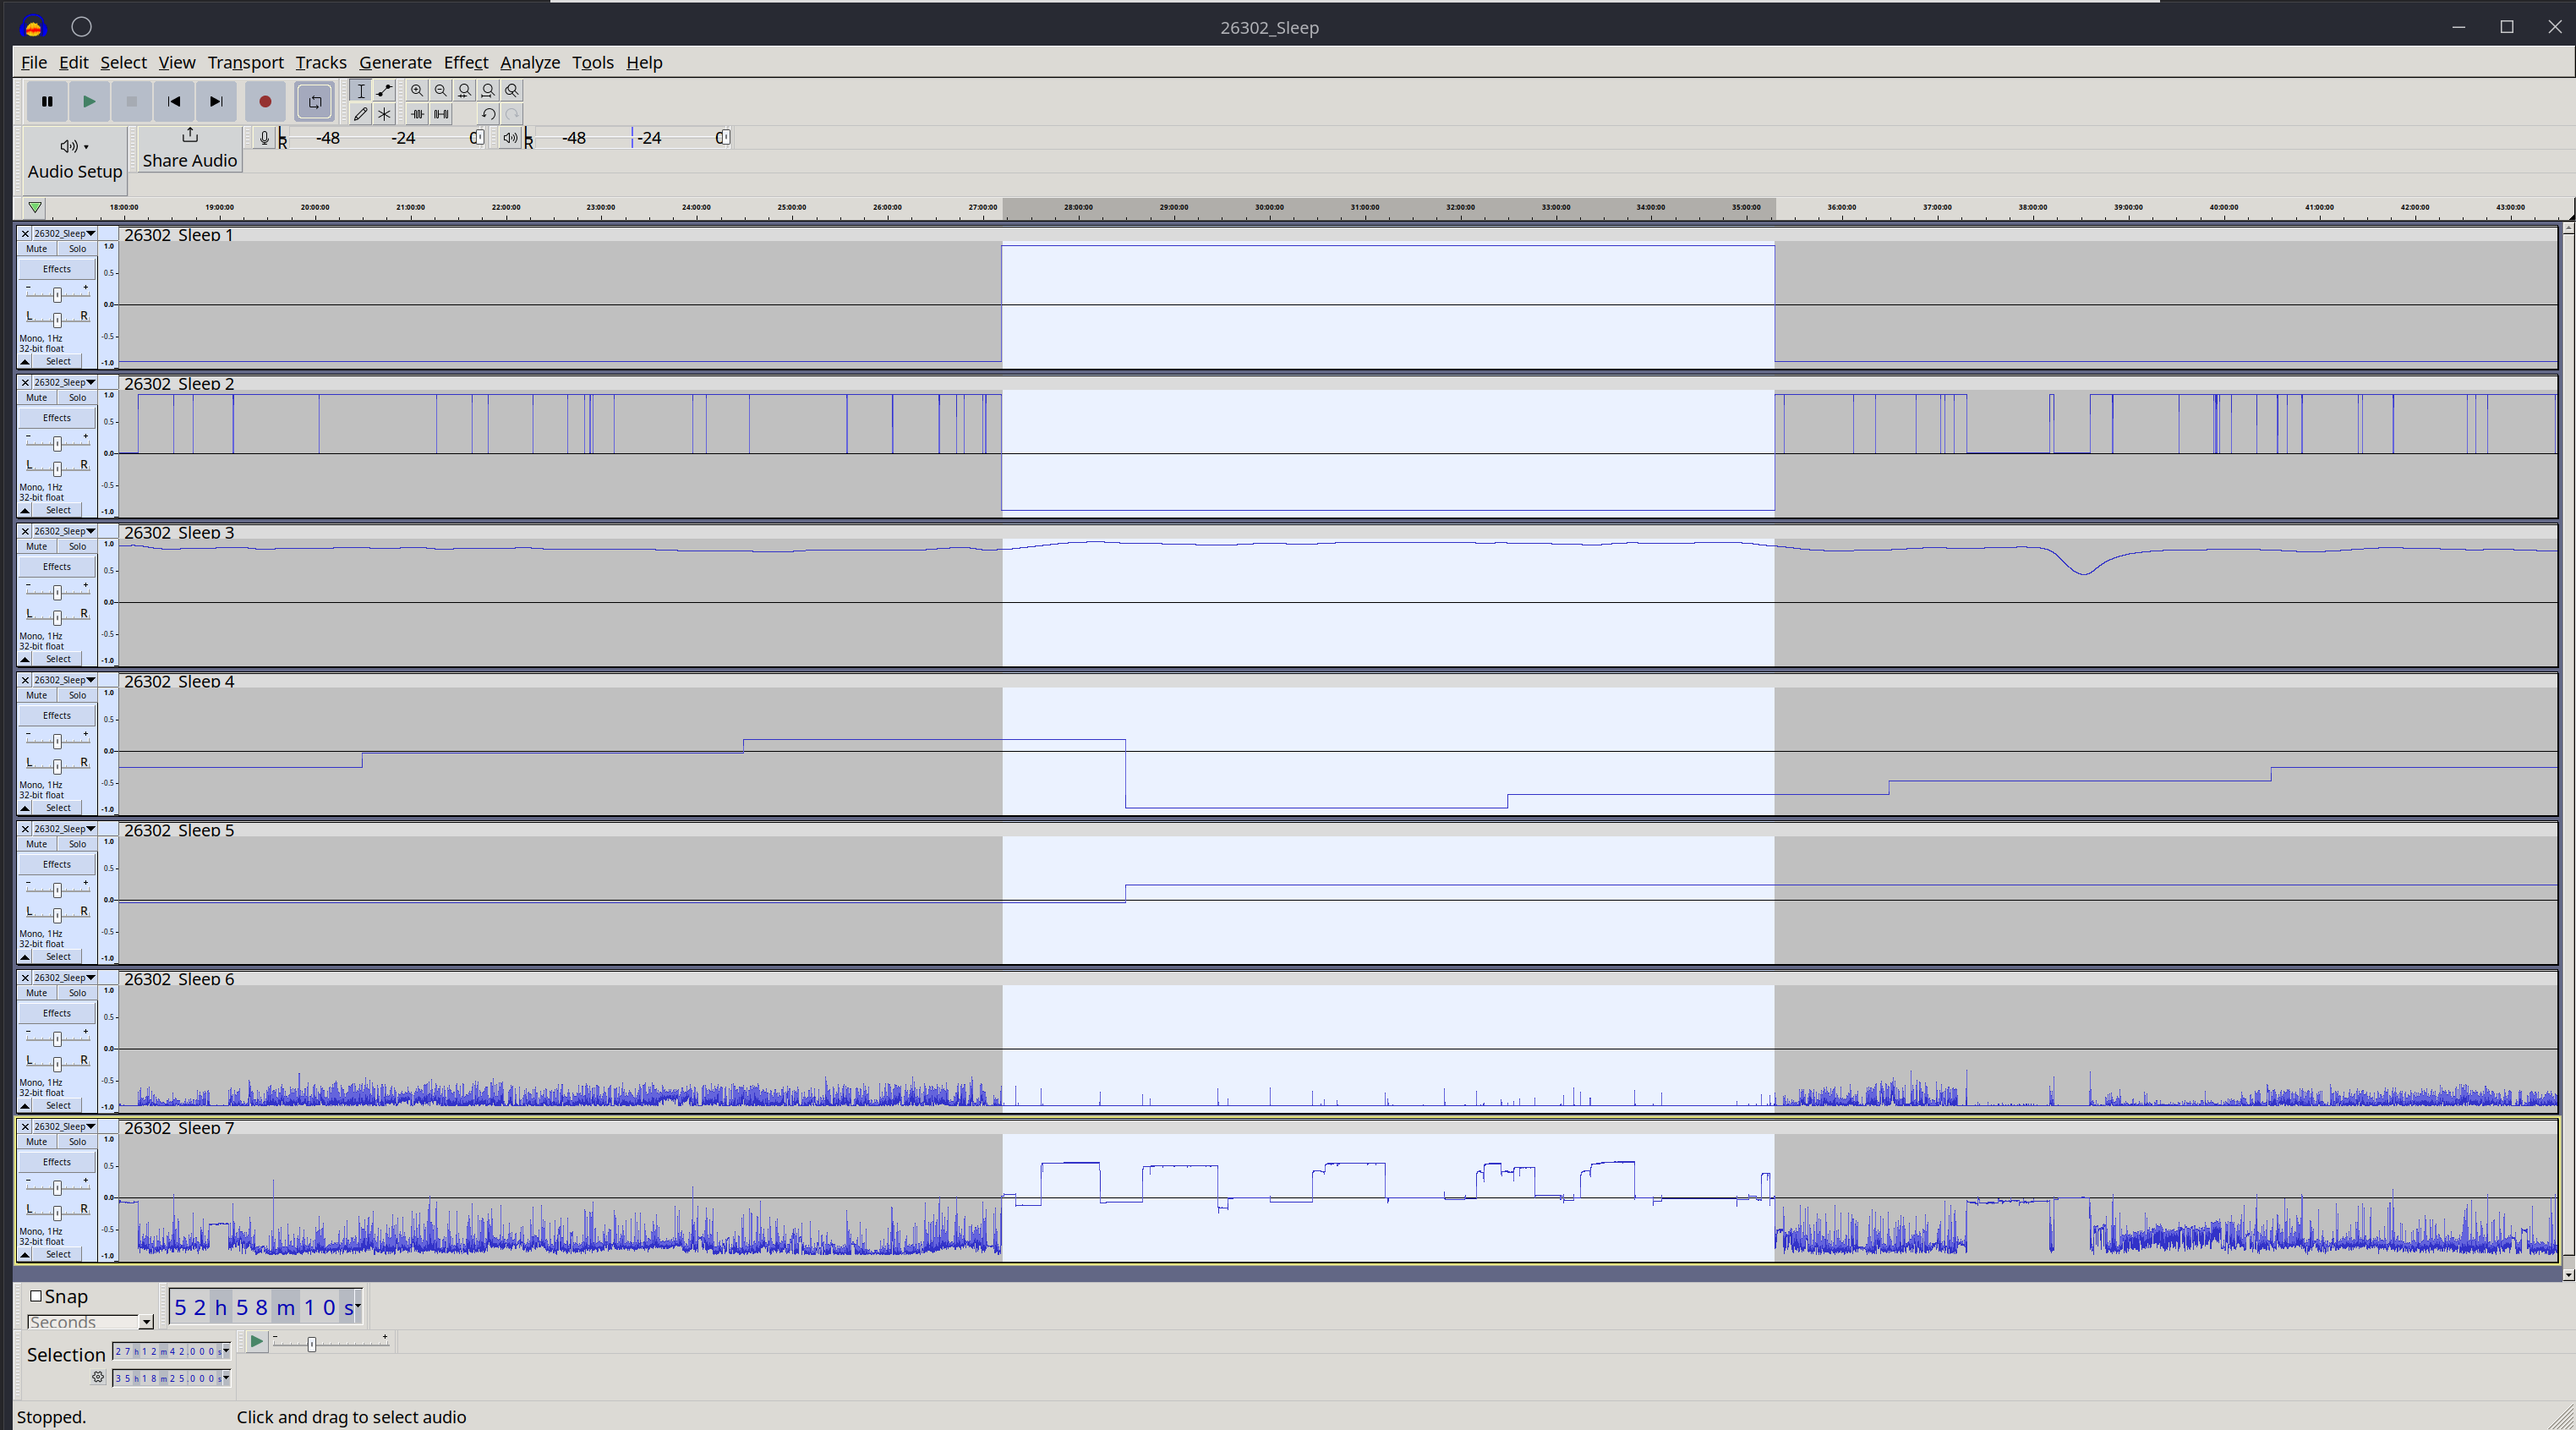
\includegraphics{figures/audacity_single_night.png}

}

\caption{\label{fig-screen_night}Screenshot of the Audacity interface
when zoomed in on a single night for the labeling of the in-bed period.
The seven horizontal panels represent the included signal features. See
Table~\ref{tbl-man_signal_features} for a detailed description of
features.}

\end{figure}

\hypertarget{annotation-process-conducted-by-expert-raters}{%
\subsubsection{Annotation Process Conducted by Expert
Raters}\label{annotation-process-conducted-by-expert-raters}}

Three experienced researchers, well-versed in working with accelerometer
data, were chosen as raters. Their proficiency ensured that they had the
requisite knowledge to accurately interpret the various data channels
presented to them. Each rater meticulously reviewed and labeled each
wav-file, marking specific timestamps that indicated in-bed and
out-of-bed activities. These annotations were then saved as individual
text files. For ensuring consistency and reliability in the annotations,
each wav-file underwent two rounds of labeling. Importantly, at no point
during this process were the raters privy to any prior annotations,
either made by themselves or their colleagues.

\hypertarget{establishing-the-ground-truth-using-zm}{%
\subsubsection{Establishing the Ground Truth Using
ZM}\label{establishing-the-ground-truth-using-zm}}

The definitive ground truth for in-bed and out-of-bed time frames was
gleaned from the sleep staging data derived from the ZM. This was
established by identifying the first and last events at night that did
not present any sensor-related issues. Nights where the ZM detected
sensor problems, either at the onset or conclusion of the recording,
were excluded from further consideration. Such sensor issues typically
arise due to inadequate attachment of electrodes. To maintain accuracy
in data collection, all participants were meticulously instructed to
affix the ZM and activate it precisely at their bedtime and to detach it
upon waking. These crucial timestamps were then utilized as the ground
truth for the study.

\hypertarget{statistical-analysis}{%
\subsubsection{Statistical Analysis}\label{statistical-analysis}}

The statistical interpretations for this study were achieved using the R
statistical software (version 4.0.2, released on 22 June 2020) and its
complementary interface, RStudio (version 1.1.456). For continuous
variables, the descriptive attributes were gauged using medians and
interquartile ranges. Meanwhile, categorical variables were assessed
based on their proportions. To offer a clear distinction, the
characteristics for children and adults were presented separately.

The core of the statistical analysis encompassed agreement studies which
were executed using the intraclass correlation coefficient (ICC) and the
Bland--Altman analysis. Additionally, to provide a comprehensive visual
representation of the agreement and symmetry across methodologies,
probability density distribution plots were integrated. The ICC, as a
metric, goes beyond merely correlating two techniques; it evaluates if
they align in magnitude. The scale for interpretation is as follows:

\(ICC < 0.5\) signifies poor agreement

\(0.5 < ICC > 0.75\) indicates moderate agreement

\(0.75 < ICC > 0.9\) represents good agreement

\(ICC > 0.90\) underscores excellent agreemen

In this research, the ICC values were interpreted based on their 95\%
confidence intervals, adhering to recommended
guidelines\textsuperscript{\protect\hyperlink{ref-koo_guideline_2016}{46}}.
The Bland--Altman analysis, on the other hand, is a tool to measure the
concurrence between two measuring
techniques\textsuperscript{\protect\hyperlink{ref-bland_measuring_1999}{47}}.
It calculates the average of the differences (representing bias) between
the two methods, and also establishes the limits of this agreement. A
positive mean difference suggests an earlier underestimation of the
in-bed or out-of-bed timestamp relative to the ZM, while a negative
difference indicates a later overestimation.

\hypertarget{results}{%
\subsection{Results}\label{results}}

Descriptive characteristics of the included subjects of the current
study are reported in Table~\ref{tbl-man_describe}.

\begingroup

\footnotesize

\hypertarget{tbl-man_describe}{}
\begin{longtable}{ll}
\caption{\label{tbl-man_describe}Descriptive characteristics of the study participants. ISCE:
International Standard Classification of Education }\tabularnewline

\toprule
Characteristic &  \\ 
\midrule
\multicolumn{2}{l}{Children} \\ 
\midrule
N & 14 \\ 
Gender (\% female) & 28.6 \\ 
Age (years) & 9 (7–10) \\ 
\midrule
\multicolumn{2}{l}{Adults} \\ 
\midrule
N & 19 \\ 
Gender (\% female) & 57.9 \\ 
Age (years) & 42 (39–46) \\ 
Education Level &  \\ 
0–3 (\%) & 36.8 \\ 
4–6 (\%) & 47.4 \\ 
7–8 (\%) & 15.8 \\ 
\bottomrule
\end{longtable}

\endgroup

\hypertarget{intraclass-correlation-coefficient-analyses}{%
\subsubsection{Intraclass Correlation Coefficient
Analyses}\label{intraclass-correlation-coefficient-analyses}}

The analyses of Intra-Class Correlation (ICC) underscored an exemplary
consistency when comparing ZM's automatic in-bed annotations with manual
annotations. This was evident in both metrics assessed: time to bed and
time out of bed. The high agreement was consistent across both
evaluation phases---Round 1 and Round 2---and was observed in the
initial baseline as well as the subsequent follow-up assessments.
Reinforcing the robustness of these findings, the lower bounds of the
confidence intervals consistently remained above 0.9, suggesting a high
degree of reliability in the agreement. For a detailed breakdown of
these results, please refer to Table~\ref{tbl-man_icc_zm_man}.

\newpage

\begingroup

\footnotesize

\hypertarget{tbl-man_icc_zm_man}{}
\begin{longtable}{llrl}
\caption{\label{tbl-man_icc_zm_man}Intraclass correlation coefficients between ZM and the average of the
manual annotations between the three raters. }\tabularnewline

\toprule
Action &  & ICC & 95\% CI \\ 
\midrule
\multicolumn{4}{l}{Baseline (n = 94 Nights)} \\ 
\midrule
To bed & Round 1 & 0.98 & (0.98; 0.99) \\ 
To bed & Round 2 & 0.98 & (0.96; 0.98) \\ 
Out of bed & Round 1 & 0.98 & (0.97; 0.99) \\ 
Out of bed & Round 2 & 0.98 & (0.96; 0.98) \\ 
\midrule
\multicolumn{4}{l}{Follow-Up (n = 54 Nights)} \\ 
\midrule
To bed & Round 1 & 0.96 & (0.94; 0.98) \\ 
To bed & Round 2 & 0.95 & (0.92; 0.97) \\ 
Out of bed & Round 1 & 0.98 & (0.97; 0.99) \\ 
Out of bed & Round 2 & 0.97 & (0.95; 0.98) \\ 
\bottomrule
\end{longtable}

\endgroup

In our analysis, we also identified a remarkable consistency between the
data from self-reports and the ZM measurements. This high level of
agreement was evident in both the initial baseline data as well as the
subsequent follow-up data. The strength of this agreement is underscored
by the fact that the lower limit of the 95\% confidence interval never
fell below a value of 0.94. For a detailed representation of this,
please refer to Table~\ref{tbl-man_icc_zm_self}.

\begingroup

\footnotesize

\hypertarget{tbl-man_icc_zm_self}{}
\begin{longtable}{lll}
\caption{\label{tbl-man_icc_zm_self}Intraclass correlation coefficients between self-report and ZM. }\tabularnewline

\toprule
 & Baseline (N = 94) & Followup (N = 54) \\ 
\cmidrule(lr){2-2} \cmidrule(lr){3-3}
 & ICC (95\% CI) &  ICC (95\% CI) \\ 
\midrule
To bed & 0.98 (0.98; 0.99) & 0.96 (0.94; 0.98) \\ 
Out of bed & 0.98 (0.97; 0.99) & 0.98 (0.96; 0.99) \\ 
\bottomrule
\end{longtable}

\endgroup

Our analysis evaluated the agreement among three manual raters in
annotating timestamps for both `to bed' and `out of bed' events. The
Intraclass Correlation Coefficients (ICCs) from this evaluation
demonstrated strong consensus among the raters. Specifically, the lower
bounds of the 95\% confidence intervals were consistently strong, never
dropping below 0.88, highlighting both good and excellent agreement
levels. However, when analyzing the ICCs more closely, subtle variations
appear between the `to bed' and `out of bed' timestamps. This nuanced
observation is detailed in Table~\ref{tbl-man_icc_man_man}.

\begingroup

\footnotesize

\hypertarget{tbl-man_icc_man_man}{}
\begin{longtable}{lll}
\caption{\label{tbl-man_icc_man_man}Intraclass correlation coefficients between manual raters. }\tabularnewline

\toprule
 & Round & ICC (95\% CI) \\ 
\midrule
\multicolumn{3}{l}{Baseline} \\ 
\midrule
To bed & Round 1 & 0.91 (0.88; 0.94) \\ 
Out of bed & Round 1 & 0.93 (0.9; 0.95) \\ 
To bed & Round 2 & 0.92 (0.89; 0.94) \\ 
Out of bed & Round 2 & 0.97 (0.96; 0.98) \\ 
\midrule
\multicolumn{3}{l}{Follow-Up} \\ 
\midrule
To bed & Round 1 & 0.94 (0.9; 0.96) \\ 
Out of bed & Round 1 & 0.97 (0.96; 0.98) \\ 
To bed & Round 2 & 0.97 (0.95; 0.98) \\ 
Out of bed & Round 2 & 0.98 (0.98; 0.99) \\ 
\bottomrule
\end{longtable}

\endgroup

The test-retest reliability exhibited good to excellent ICC agreement
for each rater between the first and second rounds, applicable to both
baseline and follow-up data (refer to
Table~\ref{tbl-man_icc_test_retest}). This robust reliability is further
evidenced by the 95\% confidence intervals having lower limits not less
than 0.86. While the ICCs across raters are broadly consistent, there's
a distinction: Raters 1 and 3 had slightly reduced agreement in their
baseline to-bed annotations relative to subsequent ones. In contrast,
Rater 2's ICC scores remained stable and didn't reflect this trend.

\begingroup

\footnotesize

\hypertarget{tbl-man_icc_test_retest}{}
\begin{longtable}{lcccc}
\caption{\label{tbl-man_icc_test_retest}Test--retest intraclass correlation coefficients between the first and
second round of manual annotations. }\tabularnewline

\toprule
 & \multicolumn{2}{c}{Baseline (N = 110)} & \multicolumn{2}{c}{Followup (N = 62)} \\ 
\cmidrule(lr){2-3} \cmidrule(lr){4-5}
 & To Bed
ICC (CI 95\%) & Out of Bed
ICC (CI 95\%) & To Bed
ICC (CI 95\%) & Out of Bed
ICC (CI 95\%) \\ 
\midrule
Rater 1 & 0.91 (0.87; 0.94) & 0.98 (0.98; 0.99) & 0.96 (0.94; 0.98) & 1 (0.99; 1) \\ 
Rater 2 & 0.97 (0.96; 0.98) & 0.91 (0.87; 0.94) & 0.91 (0.86; 0.95) & 0.99 (0.98; 0.99) \\ 
Rater 3 & 0.91 (0.87; 0.94) & 0.96 (0.94; 0.97) & 0.98 (0.97; 0.99) & 0.98 (0.97; 0.99) \\ 
\bottomrule
\end{longtable}

\endgroup

\hypertarget{bland-altman-analyses}{%
\subsubsection{Bland-Altman Analyses}\label{bland-altman-analyses}}

Table~\ref{tbl-7} presents the bias and its corresponding confidence
intervals, as well as the upper and lower limits of agreement, comparing
manual annotation and self-report to ZM. The bias for manual annotation
relative to ZM ranges from -6 minutes to 5 minutes. In contrast, the
self-report exhibits a slightly smaller bias when compared to ZM.
Notably, the magnitude of the limits of agreement appears consistent
across both methods of comparison.

\begingroup

\footnotesize

\hypertarget{tbl-7}{}
\begin{longtable}{lccc}
\caption{\label{tbl-7}Bland--Altman analysis was conducted to assess the inter-method
agreement. This analysis compared manual annotation to ZM and also
compared self-report to ZM. All the measurements in the analysis are
presented in minutes. }\tabularnewline

\toprule
Method & Bias & Lower\_LOA & Upper\_LOA \\ 
\midrule
\multicolumn{4}{l}{Baseline, to bed, n = 94} \\ 
\midrule
Manual, round 1 & 3.02 (-0.44; 6.47) & 36.07 (30.15; 42) & -30.04 (-35.96;-24.12) \\ 
Manual, round 2 & 0.48 (-2.42; 3.39) & 28.27 (23.29; 33.24) & -27.3 (-32.28;-22.32) \\ 
Self-report & 1.23 (-1.57; 4.03) & 28.02 (23.21; 32.82) & -25.56 (-30.37;-20.76) \\ 
\midrule
\multicolumn{4}{l}{Baseline, out of bed, n = 94} \\ 
\midrule
Manual, round 1 & 0.53 (-2.34; 3.4) & 27.96 (23.05; 32.88) & -26.9 (-31.82;-21.99) \\ 
Manual, round 2 & 0.98 (-1.47; 3.43) & 24.45 (20.24; 28.66) & -22.49 (-26.7;-18.28) \\ 
Self-report & -2.79 (-5.26; -0.32) & 20.87 (16.63; 25.11) & -26.45 (-30.69;-22.21) \\ 
\midrule
\multicolumn{4}{l}{Follow-up, to bed, n = 54} \\ 
\midrule
Manual, round 1 & -6.08 (-11.34; -0.83) & 31.64 (22.61; 40.67) & -43.81 (-52.84;-34.77) \\ 
Manual, round 2 & -0.4 (-5.3; 4.51) & 34.8 (26.37; 43.23) & -35.6 (-44.03;-27.17) \\ 
Self-report & 0.77 (-4.08; 5.62) & 35.59 (27.25; 43.93) & -34.06 (-42.4;-25.72) \\ 
\midrule
\multicolumn{4}{l}{Follow-up, out of bed, n = 54} \\ 
\midrule
Manual, round 1 & 4.95 (0.65; 9.25) & 35.85 (28.45; 43.25) & -25.95 (-33.35;-18.55) \\ 
Manual, round 2 & 2.57 (-0.76; 5.89) & 26.44 (20.72; 32.15) & -21.3 (-27.02;-15.59) \\ 
Self-report & 0.56 (-3.62; 4.74) & 30.57 (23.39; 37.76) & -29.45 (-36.64;-22.26) \\ 
\bottomrule
\end{longtable}

\endgroup

\newpage

\hypertarget{references}{%
\section{References}\label{references}}

\hypertarget{refs}{}
\begin{CSLReferences}{0}{0}
\leavevmode\vadjust pre{\hypertarget{ref-kraus_physical_2019}{}}%
\CSLLeftMargin{1. }%
\CSLRightInline{Kraus, W. E. \emph{et al.} Physical activity, all-cause
and cardiovascular mortality, and cardiovascular disease. \emph{Med Sci
Sports Exerc} \textbf{51}, 1270--1281 (2019)
doi:\href{https://doi.org/10.1249/MSS.0000000000001939}{10.1249/MSS.0000000000001939}.}

\leavevmode\vadjust pre{\hypertarget{ref-lee_effect_2012}{}}%
\CSLLeftMargin{2. }%
\CSLRightInline{Lee, I.-M. \emph{et al.} Effect of physical inactivity
on major non-communicable diseases worldwide: An analysis of burden of
disease and life expectancy. \emph{Lancet} \textbf{380}, 219--229 (2012)
doi:\href{https://doi.org/10.1016/S0140-6736(12)61031-9}{10.1016/S0140-6736(12)61031-9}.}

\leavevmode\vadjust pre{\hypertarget{ref-wilmot_sedentary_2012}{}}%
\CSLLeftMargin{3. }%
\CSLRightInline{Wilmot, E. G. \emph{et al.} Sedentary time in adults and
the association with diabetes, cardiovascular disease and death:
Systematic review and meta-analysis. \emph{Diabetologia} \textbf{55},
2895--2905 (2012) URL: \url{https://doi.org/10.1007/s00125-012-2677-z}
Accessed 5 August 2023, 2023:2023.}

\leavevmode\vadjust pre{\hypertarget{ref-cappuccio_sleep_2010}{}}%
\CSLLeftMargin{4. }%
\CSLRightInline{Cappuccio, F. P., D'Elia, L., Strazzullo, P. \& Miller,
M. A. Sleep duration and all-cause mortality: A systematic review and
meta-analysis of prospective studies. \emph{Sleep} \textbf{33}, 585--592
(2010)
doi:\href{https://doi.org/10.1093/sleep/33.5.585}{10.1093/sleep/33.5.585}.}

\leavevmode\vadjust pre{\hypertarget{ref-kl_physical_2018}{}}%
\CSLLeftMargin{5. }%
\CSLRightInline{Kl, P. \emph{et al.} The physical activity guidelines
for americans. \emph{{JAMA}} \textbf{320}, (2018) URL:
\url{https://pubmed.ncbi.nlm.nih.gov/30418471/} Accessed 5 August 2023,
2023:2023.}

\leavevmode\vadjust pre{\hypertarget{ref-el-zine_fysisk_nodate-1}{}}%
\CSLLeftMargin{6. }%
\CSLRightInline{El-Zine, H. Fysisk aktivitet for voksne (18-64 år).}

\leavevmode\vadjust pre{\hypertarget{ref-el-zine_fysisk_nodate}{}}%
\CSLLeftMargin{7. }%
\CSLRightInline{El-Zine, H. Fysisk aktivitet for børn og unge (5-17
år).}

\leavevmode\vadjust pre{\hypertarget{ref-liguori_evolving_2023}{}}%
\CSLLeftMargin{8. }%
\CSLRightInline{Liguori, C. \emph{et al.} The evolving role of
quantitative actigraphy in clinical sleep medicine. \emph{Sleep Medicine
Reviews} \textbf{68}, 101762 (2023) URL:
\url{https://www.sciencedirect.com/science/article/pii/S1087079223000187}
Accessed 26 June 2023, 2023:2023.}

\leavevmode\vadjust pre{\hypertarget{ref-biddle_physical_2011}{}}%
\CSLLeftMargin{9. }%
\CSLRightInline{Biddle, S. J. H. \& Asare, M. Physical activity and
mental health in children and adolescents: A review of reviews. \emph{Br
J Sports Med} \textbf{45}, 886--895 (2011)
doi:\href{https://doi.org/10.1136/bjsports-2011-090185}{10.1136/bjsports-2011-090185}.}

\leavevmode\vadjust pre{\hypertarget{ref-warburton_health_2017}{}}%
\CSLLeftMargin{10. }%
\CSLRightInline{Warburton, D. E. R. \& Bredin, S. S. D. Health benefits
of physical activity: A systematic review of current systematic reviews.
\emph{Curr Opin Cardiol} \textbf{32}, 541--556 (2017)
doi:\href{https://doi.org/10.1097/HCO.0000000000000437}{10.1097/HCO.0000000000000437}.}

\leavevmode\vadjust pre{\hypertarget{ref-strath_guide_2013}{}}%
\CSLLeftMargin{11. }%
\CSLRightInline{Strath, S. J. \emph{et al.} Guide to the assessment of
physical activity: Clinical and research applications: A scientific
statement from the american heart association. \emph{Circulation}
\textbf{128}, 2259--2279 (2013)
doi:\href{https://doi.org/10.1161/01.cir.0000435708.67487.da}{10.1161/01.cir.0000435708.67487.da}.}

\leavevmode\vadjust pre{\hypertarget{ref-arem_leisure_2015}{}}%
\CSLLeftMargin{12. }%
\CSLRightInline{Arem, H. \emph{et al.} Leisure time physical activity
and mortality: A detailed pooled analysis of the dose-response
relationship. \emph{{JAMA} Intern Med} \textbf{175}, 959--967 (2015)
doi:\href{https://doi.org/10.1001/jamainternmed.2015.0533}{10.1001/jamainternmed.2015.0533}.}

\leavevmode\vadjust pre{\hypertarget{ref-rollo_whole_2020}{}}%
\CSLLeftMargin{13. }%
\CSLRightInline{Rollo, S., Antsygina, O. \& Tremblay, M. S. The whole
day matters: Understanding 24-hour movement guideline adherence and
relationships with health indicators across the lifespan. \emph{Journal
of Sport and Health Science} \textbf{9}, 493--510 (2020) URL:
\url{https://www.sciencedirect.com/science/article/pii/S2095254620300910}
Accessed 5 August 2023, 2023:2023.}

\leavevmode\vadjust pre{\hypertarget{ref-rosenberger_24-hour_2019}{}}%
\CSLLeftMargin{14. }%
\CSLRightInline{Rosenberger, M. E. \emph{et al.} The 24-hour activity
cycle: A new paradigm for physical activity. \emph{Med Sci Sports Exerc}
\textbf{51}, 454--464 (2019)
doi:\href{https://doi.org/10.1249/MSS.0000000000001811}{10.1249/MSS.0000000000001811}.}

\leavevmode\vadjust pre{\hypertarget{ref-paruthi_consensus_2016}{}}%
\CSLLeftMargin{15. }%
\CSLRightInline{Paruthi, S. \emph{et al.} Consensus statement of the
american academy of sleep medicine on the recommended amount of sleep
for healthy children: Methodology and discussion. \emph{J Clin Sleep
Med} \textbf{12}, 1549--1561 (2016)
doi:\href{https://doi.org/10.5664/jcsm.6288}{10.5664/jcsm.6288}.}

\leavevmode\vadjust pre{\hypertarget{ref-tremblay_sedentary_2017}{}}%
\CSLLeftMargin{16. }%
\CSLRightInline{Tremblay, M. S. \emph{et al.} Sedentary behavior
research network ({SBRN}) -- terminology consensus project process and
outcome. \emph{International Journal of Behavioral Nutrition and
Physical Activity} \textbf{14}, 75 (2017) URL:
\url{https://doi.org/10.1186/s12966-017-0525-8} Accessed 5 August 2023,
2023:2023.}

\leavevmode\vadjust pre{\hypertarget{ref-welk_reliability_2004}{}}%
\CSLLeftMargin{17. }%
\CSLRightInline{Welk, G. J., Schaben, J. A. \& Morrow, J. R.
\href{https://www.ncbi.nlm.nih.gov/pubmed/15354049}{Reliability of
accelerometry-based activity monitors: A generalizability study}.
\emph{Med Sci Sports Exerc} \textbf{36}, 1637--1645 (2004).}

\leavevmode\vadjust pre{\hypertarget{ref-migueles_comparability_2019}{}}%
\CSLLeftMargin{18. }%
\CSLRightInline{Migueles, J. H. \emph{et al.} Comparability of
accelerometer signal aggregation metrics across placements and dominant
wrist cut points for the assessment of physical activity in adults.
\emph{Sci Rep} \textbf{9}, 18235 (2019) URL:
\url{https://www.nature.com/articles/s41598-019-54267-y} Accessed 5
August 2023, 2023:2023.}

\leavevmode\vadjust pre{\hypertarget{ref-hastie01statisticallearning}{}}%
\CSLLeftMargin{19. }%
\CSLRightInline{Hastie, T., Tibshirani, R. \& Friedman, J. \emph{The
elements of statistical learning}. (Springer New York Inc., 2001).}

\leavevmode\vadjust pre{\hypertarget{ref-fiorillo_automated_2019}{}}%
\CSLLeftMargin{20. }%
\CSLRightInline{Fiorillo, L. \emph{et al.} Automated sleep scoring: A
review of the latest approaches. \emph{Sleep Med Rev} \textbf{48},
101204 (2019)
doi:\href{https://doi.org/10.1016/j.smrv.2019.07.007}{10.1016/j.smrv.2019.07.007}.}

\leavevmode\vadjust pre{\hypertarget{ref-van_der_ploeg_modern_2014}{}}%
\CSLLeftMargin{21. }%
\CSLRightInline{Ploeg, T. van der, Austin, P. C. \& Steyerberg, E. W.
Modern modelling techniques are data hungry: A simulation study for
predicting dichotomous endpoints. \emph{{BMC} Med Res Methodol}
\textbf{14}, 137 (2014)
doi:\href{https://doi.org/10.1186/1471-2288-14-137}{10.1186/1471-2288-14-137}.}

\leavevmode\vadjust pre{\hypertarget{ref-chaput_systematic_2017}{}}%
\CSLLeftMargin{22. }%
\CSLRightInline{Chaput, J.-P. \emph{et al.} Systematic review of the
relationships between sleep duration and health indicators in the early
years (0-4~years). \emph{{BMC} Public Health} \textbf{17}, 855 (2017)
doi:\href{https://doi.org/10.1186/s12889-017-4850-2}{10.1186/s12889-017-4850-2}.}

\leavevmode\vadjust pre{\hypertarget{ref-chaput_systematic_2016}{}}%
\CSLLeftMargin{23. }%
\CSLRightInline{Chaput, J.-P. \emph{et al.} Systematic review of the
relationships between sleep duration and health indicators in
school-aged children and youth. \emph{Appl Physiol Nutr Metab}
\textbf{41}, S266--282 (2016)
doi:\href{https://doi.org/10.1139/apnm-2015-0627}{10.1139/apnm-2015-0627}.}

\leavevmode\vadjust pre{\hypertarget{ref-st-onge_sleep_2016}{}}%
\CSLLeftMargin{24. }%
\CSLRightInline{St-Onge, M.-P. \emph{et al.} Sleep duration and quality:
Impact on lifestyle behaviors and cardiometabolic health: A scientific
statement from the american heart association. \emph{Circulation}
\textbf{134}, e367--e386 (2016)
doi:\href{https://doi.org/10.1161/CIR.0000000000000444}{10.1161/CIR.0000000000000444}.}

\leavevmode\vadjust pre{\hypertarget{ref-gruber_position_2014}{}}%
\CSLLeftMargin{25. }%
\CSLRightInline{Gruber, R. \emph{et al.}
\href{https://www.ncbi.nlm.nih.gov/pmc/articles/PMC4197518}{Position
statement on pediatric sleep for psychiatrists}. \emph{J Can Acad Child
Adolesc Psychiatry} \textbf{23}, 174--195 (2014).}

\leavevmode\vadjust pre{\hypertarget{ref-haghayegh_application_2020}{}}%
\CSLLeftMargin{26. }%
\CSLRightInline{Haghayegh, S., Khoshnevis, S., Smolensky, M. H. \&
Diller, K. R. Application of deep learning to improve sleep scoring of
wrist actigraphy. \emph{Sleep Med} \textbf{74}, 235--241 (2020)
doi:\href{https://doi.org/10.1016/j.sleep.2020.05.008}{10.1016/j.sleep.2020.05.008}.}

\leavevmode\vadjust pre{\hypertarget{ref-vaughn_technical_2008}{}}%
\CSLLeftMargin{27. }%
\CSLRightInline{Vaughn, B. V. \& Giallanza, P. Technical review of
polysomnography. \emph{Chest} \textbf{134}, 1310--1319 (2008)
doi:\href{https://doi.org/10.1378/chest.08-0812}{10.1378/chest.08-0812}.}

\leavevmode\vadjust pre{\hypertarget{ref-sundararajan_sleep_2021}{}}%
\CSLLeftMargin{28. }%
\CSLRightInline{Sundararajan, K. \emph{et al.} Sleep classification from
wrist-worn accelerometer data using random forests. \emph{Sci Rep}
\textbf{11}, 24 (2021) URL:
\url{https://www.nature.com/articles/s41598-020-79217-x} Accessed 13
June 2023, 2023:2023.}

\leavevmode\vadjust pre{\hypertarget{ref-van_de_water_objective_2011}{}}%
\CSLLeftMargin{29. }%
\CSLRightInline{Van De Water, A. T. M., Holmes, A. \& Hurley, D. A.
Objective measurements of sleep for non-laboratory settings as
alternatives to polysomnography -- a systematic review. \emph{Journal of
Sleep Research} \textbf{20}, 183--200 (2011) URL:
\url{https://onlinelibrary.wiley.com/doi/abs/10.1111/j.1365-2869.2009.00814.x}
Accessed 21 June 2023, 2023:2023.}

\leavevmode\vadjust pre{\hypertarget{ref-younes_staging_2016}{}}%
\CSLLeftMargin{30. }%
\CSLRightInline{Younes, M., Raneri, J. \& Hanly, P. Staging sleep in
polysomnograms: Analysis of inter-scorer variability. \emph{J Clin Sleep
Med} \textbf{12}, 885--894 (2016)
doi:\href{https://doi.org/10.5664/jcsm.5894}{10.5664/jcsm.5894}.}

\leavevmode\vadjust pre{\hypertarget{ref-dafna_sleep-wake_2015}{}}%
\CSLLeftMargin{31. }%
\CSLRightInline{Dafna, E., Tarasiuk, A. \& Zigel, Y. Sleep-wake
evaluation from whole-night non-contact audio recordings of breathing
sounds. \emph{{PLOS} {ONE}} \textbf{10}, e0117382 (2015) URL:
\url{https://journals.plos.org/plosone/article?id=10.1371/journal.pone.0117382}
Accessed 5 August 2023, 2023:2023.}

\leavevmode\vadjust pre{\hypertarget{ref-montazeri_ghahjaverestan_sleepwakefulness_2020}{}}%
\CSLLeftMargin{32. }%
\CSLRightInline{Montazeri Ghahjaverestan, N. \emph{et al.}
Sleep/wakefulness detection using tracheal sounds and movements.
\emph{Nat Sci Sleep} \textbf{12}, 1009--1021 (2020)
doi:\href{https://doi.org/10.2147/NSS.S276107}{10.2147/NSS.S276107}.}

\leavevmode\vadjust pre{\hypertarget{ref-hees_novel_2015}{}}%
\CSLLeftMargin{33. }%
\CSLRightInline{Hees, V. T. van \emph{et al.} A novel, open access
method to assess sleep duration using a wrist-worn accelerometer.
\emph{{PLOS} {ONE}} \textbf{10}, e0142533 (2015) URL:
\url{https://journals.plos.org/plosone/article?id=10.1371/journal.pone.0142533}
Accessed 13 June 2023, 2023:2023.}

\leavevmode\vadjust pre{\hypertarget{ref-madsen_actigraphy_2013}{}}%
\CSLLeftMargin{34. }%
\CSLRightInline{Madsen, M. T., Rosenberg, J. \& Gögenur, I. Actigraphy
for measurement of sleep and sleep-wake rhythms in relation to surgery.
\emph{J Clin Sleep Med} \textbf{9}, 387--394 (2013)
doi:\href{https://doi.org/10.5664/jcsm.2598}{10.5664/jcsm.2598}.}

\leavevmode\vadjust pre{\hypertarget{ref-schwab_actigraphy_2018}{}}%
\CSLLeftMargin{35. }%
\CSLRightInline{Schwab, K. E. \emph{et al.} Actigraphy to evaluate sleep
in the intensive care unit. A systematic review. \emph{Ann Am Thorac
Soc} \textbf{15}, 1075--1082 (2018)
doi:\href{https://doi.org/10.1513/AnnalsATS.201801-004OC}{10.1513/AnnalsATS.201801-004OC}.}

\leavevmode\vadjust pre{\hypertarget{ref-barouni_ambulatory_2020}{}}%
\CSLLeftMargin{36. }%
\CSLRightInline{Barouni, A. \emph{et al.} Ambulatory sleep scoring using
accelerometers-distinguishing between nonwear and sleep/wake states.
\emph{{PeerJ}} \textbf{8}, e8284 (2020)
doi:\href{https://doi.org/10.7717/peerj.8284}{10.7717/peerj.8284}.}

\leavevmode\vadjust pre{\hypertarget{ref-skovgaard_manual_2021}{}}%
\CSLLeftMargin{37. }%
\CSLRightInline{Skovgaard, E. L., Pedersen, J., Møller, N. C., Grøntved,
A. \& Brønd, J. C. Manual annotation of time in bed using free-living
recordings of accelerometry data. \emph{Sensors (Basel)} \textbf{21},
8442 (2021)
doi:\href{https://doi.org/10.3390/s21248442}{10.3390/s21248442}.}

\leavevmode\vadjust pre{\hypertarget{ref-rasmussen_feasibility_2021}{}}%
\CSLLeftMargin{38. }%
\CSLRightInline{Rasmussen, M. G. B. \emph{et al.} Feasibility of two
screen media reduction interventions: Results from the {SCREENS} pilot
trial. \emph{{PLOS} {ONE}} \textbf{16}, e0259657 (2021) URL:
\url{https://journals.plos.org/plosone/article?id=10.1371/journal.pone.0259657}
Accessed 12 June 2023, 2023:2023.}

\leavevmode\vadjust pre{\hypertarget{ref-rasmussen_short-term_2020}{}}%
\CSLLeftMargin{39. }%
\CSLRightInline{Rasmussen, M. G. B. \emph{et al.} Short-term efficacy of
reducing screen media use on physical activity, sleep, and physiological
stress in families with children aged 4--14: Study protocol for the
{SCREENS} randomized controlled trial. \emph{{BMC} Public Health}
\textbf{20}, 380 (2020) URL:
\url{https://doi.org/10.1186/s12889-020-8458-6} Accessed 12 June 2023,
2023:2023.}

\leavevmode\vadjust pre{\hypertarget{ref-pedersen_self-administered_2021}{}}%
\CSLLeftMargin{40. }%
\CSLRightInline{Pedersen, J., Rasmussen, M. G. B., Olesen, L. G.,
Kristensen, P. L. \& Grøntved, A. Self-administered
electroencephalography-based sleep assessment: Compliance and perceived
feasibility in children and adults. \emph{Sleep Science and Practice}
\textbf{5}, 8 (2021) URL:
\url{https://doi.org/10.1186/s41606-021-00059-1} Accessed 22 June 2023,
2023:2023.}

\leavevmode\vadjust pre{\hypertarget{ref-jaeschke_variability_2018}{}}%
\CSLLeftMargin{41. }%
\CSLRightInline{Jaeschke, L., Steinbrecher, A., Jeran, S., Konigorski,
S. \& Pischon, T. Variability and reliability study of overall physical
activity and activity intensity levels using 24~h-accelerometry-assessed
data. \emph{{BMC} Public Health} \textbf{18}, 530 (2018) URL:
\url{https://doi.org/10.1186/s12889-018-5415-8} Accessed 5 August 2023,
2023:2023.}

\leavevmode\vadjust pre{\hypertarget{ref-wang_evaluation_2015}{}}%
\CSLLeftMargin{42. }%
\CSLRightInline{Wang, Y., Loparo, K. A., Kelly, M. R. \& Kaplan, R. F.
Evaluation of an automated single-channel sleep staging algorithm.
\emph{Nat Sci Sleep} \textbf{7}, 101--111 (2015) URL:
\url{https://www.ncbi.nlm.nih.gov/pmc/articles/PMC4583116/} Accessed 13
June 2023, 2023:2023.}

\leavevmode\vadjust pre{\hypertarget{ref-kaplan_performance_2014}{}}%
\CSLLeftMargin{43. }%
\CSLRightInline{Kaplan, R. F., Wang, Y., Loparo, K. A., Kelly, M. R. \&
Bootzin, R. R. Performance evaluation of an automated single-channel
sleep--wake detection algorithm. \emph{Nat Sci Sleep} \textbf{6},
113--122 (2014) URL:
\url{https://www.ncbi.nlm.nih.gov/pmc/articles/PMC4206400/} Accessed 13
June 2023, 2023:2023.}

\leavevmode\vadjust pre{\hypertarget{ref-audacity}{}}%
\CSLLeftMargin{44. }%
\CSLRightInline{Audacity Team. Audacity\textregistered{} software is
copyright © 1999--2021 audacity team. (2021).}

\leavevmode\vadjust pre{\hypertarget{ref-skotte_detection_2014}{}}%
\CSLLeftMargin{45. }%
\CSLRightInline{Skotte, J., Korshøj, M., Kristiansen, J., Hanisch, C. \&
Holtermann, A. Detection of physical activity types using triaxial
accelerometers. \emph{Journal of Physical Activity and Health}
\textbf{11}, 76--84 (2014) URL:
\url{https://journals.humankinetics.com/view/journals/jpah/11/1/article-p76.xml}
Accessed 12 June 2023, 2023:2023.}

\leavevmode\vadjust pre{\hypertarget{ref-koo_guideline_2016}{}}%
\CSLLeftMargin{46. }%
\CSLRightInline{Koo, T. K. \& Li, M. Y. A guideline of selecting and
reporting intraclass correlation coefficients for reliability research.
\emph{J Chiropr Med} \textbf{15}, 155--163 (2016)
doi:\href{https://doi.org/10.1016/j.jcm.2016.02.012}{10.1016/j.jcm.2016.02.012}.}

\leavevmode\vadjust pre{\hypertarget{ref-bland_measuring_1999}{}}%
\CSLLeftMargin{47. }%
\CSLRightInline{Bland, J. M. \& Altman, D. G. Measuring agreement in
method comparison studies. \emph{Stat Methods Med Res} \textbf{8},
135--160 (1999) URL: \url{https://doi.org/10.1177/096228029900800204}
Accessed 9 August 2023, 2023:2023.}

\end{CSLReferences}

\newpage

\hypertarget{list-of-appendices}{%
\section{List of Appendices}\label{list-of-appendices}}

\begin{itemize}
\item
  \textbf{Appendix I}: Manual Annotation of Time in Bed Using
  Free-Living Recordings of Accelerometry Data
\item
  \textbf{Appendix II}: Generalizability and performance of methods to
  detect non‑wear with free‑living accelerometer recordings
\item
  \textbf{Appendix III}: \emph{I}mproving Sleep Quality Estimation in
  Children and Adolescents: A Comparative Study of Machine Learning and
  Deep Learning Techniques Utilizing Free-Living Accelerometer Data from
  Thigh-Worn Devices and EEG-Based Sleep Tracking
\end{itemize}

\newpage

\begin{center}

\textbf{\textsf{\Huge Appendix I}}

\addcontentsline{toc}{subsection}{Appendix I}

\vspace{1cm}

\textsf{\Huge Manual Annotation of Time in Bed Using Free-Living Accelerometry Data}

\vspace{5cm}

This paper was published in \textbf{Sensors} and is used here under the terms and conditions of the Creative Commons Attribution (CC BY) license (\href{https://creativecommons.org/licenses/by/4.0/}{https://creativecommons.org/licenses/by/4.0/})

\vspace{1cm}

DOI: \href{https://doi.org/10.3390/s21248442}{https://doi.org/10.3390/s21248442}

\end{center}

\includepdf[pages=-]{my_papers/paper1.pdf}

\begin{center}

\textbf{\textsf{\Huge Appendix II}}

\addcontentsline{toc}{subsection}{Appendix II}

\vspace{1cm}

\textsf{\Huge Generalizability and Performance of Methods to Detect Non-Wear With Free-Living Accelerometer Recordings}

\vspace{5cm}

This paper was published in \textbf{Scientific Reports} and is used here under the terms and conditions of the Creative Commons Attribution (CC BY) license (\href{https://creativecommons.org/licenses/by/4.0/}{https://creativecommons.org/licenses/by/4.0/})

\vspace{1cm}

DOI: \href{https://doi.org/10.1038/s41598-023-29666-x}{https://doi.org/10.1038/s41598-023-29666-x}

\end{center}

\includepdf[pages=-]{my_papers/paper2.pdf}

\begin{center}

\textbf{\textsf{\Huge Appendix III}}

\addcontentsline{toc}{subsection}{Appendix III}

\vspace{1cm}

\textsf{\Huge Improving Sleep Quality Estimation in Children and Adolescents: A Comparative Study of Machine Learning and Deep Learning Techniques Utilizing Free-Living Accelerometer Data from Thigh-Worn Devices and EEG-Based Sleep Tracking}

\vspace{5cm}

This paper is under review in \textbf{npj Digital Medicine}.
The version presented here is a preprint of the submitted manuscript in compliance with npj Digital Medicine's self-archiving policy.

\vspace{1cm}

DOI: \href{https://doi.org/10.1038/s41598-023-29666-x}{https://doi.org/10.1038/s41598-023-29666-x}

\end{center}

\includepdf[pages=-]{my_papers/paper3.pdf}



\end{document}
